\documentclass[12pt,a4paper]{article}

\usepackage[left=1in,right=1in,top=1in,bottom=1in]{geometry}                % See geometry.pdf to learn the layout options. There are lots.
\usepackage[parfill]{parskip}    % Activate to begin paragraphs with an empty line rather than an indent
\usepackage{microtype} \hyphenpenalty=750
\usepackage{graphicx}
\usepackage{epstopdf} \DeclareGraphicsRule{.tif}{png}{.png}{`convert #1 `dirname #1`/`basename #1 .tif`.png}
% \usepackage[applemac]{inputenc}
\usepackage{booktabs}
% \usepackage{fancyhdr} \pagestyle{fancy} \chead{\hifibau} \cfoot{\thepage}
% \usepackage[english,ngerman]{babel}

\usepackage{siunitx}

\PassOptionsToPackage{hyphens}{url}\usepackage[colorlinks]{hyperref}
\usepackage{caption} \captionsetup{labelfont={sf,bf}, size=footnotesize}

\usepackage[superscript,biblabel]{cite}

% set format of document title
\usepackage{titling}
\pretitle{\begin{center}\Large\bfseries}
\posttitle{\end{center}\vspace{1em}}
\preauthor{\begin{center}\large}
\postauthor{\end{center}\vspace{1em}}
\predate{\begin{center}\large}
\postdate{\end{center}\vspace{1em}}

% set formats of section headings
\usepackage[explicit]{titlesec}
\titleformat{\title}{\centering}{\thesection.}{0.5em}{\MakeUppercase{#1}}
%\titleformat{\section}{\centering}{\thesection.}{0.5em}{\MakeUppercase{#1}}
\titleformat{\section}{}{\thesection.}{0.5em}{\MakeUppercase{#1}}
%\titleformat{\subsection}[runin]{\slshape}{\thesubsection.}{0.5em}{#1. }
\titleformat{\subsection}{\slshape}{\thesubsection.}{0.5em}{#1 }
\titleformat{\subsubsection}[runin]{\slshape}{\thesubsubsection.}{0.5em}{#1. }
 
\usepackage[T1]{fontenc} \usepackage[scaled=.90]{helvet} \renewcommand{\familydefault}{\sfdefault} \usepackage[helvet]{sfmath}

\newcommand{\Ohm}{\ensuremath{\Omega}}
\sisetup{detect-all} % tell siunitx to detect font stuff


% \setlength{\columnsep}{0.75cm} 

\graphicspath{{figures/}}

% \interfootnotelinepenalty=10000

\providecommand{\figr}[1]{Fig.~\ref{fig:#1}}
\providecommand{\figlabel}[1]{\label{fig:#1}}
\providecommand{\tabl}[1]{Tab.~\ref{tab:#1}}
\providecommand{\tablabel}[1]{\label{tab:#1}}
\providecommand{\secn}[1]{Sec.~\ref{sec:#1}}
\providecommand{\seclabel}[1]{\label{sec:#1}}


%% define formats of section and subsection etc. headings:
%    \makeatletter
%    \def\section{\@startsection{section}{1}%
%    \z@{.7\linespacing\@plus\linespacing}{.5\linespacing}%
%%    {\normalfont\bfseries\centering}}
%    {\Large\centering}}
%    
%    \def\subsection{\@startsection{subsection}{2}%
%    \z@{.5\linespacing\@plus.7\linespacing}{-.5em}%
%%    {\normalfont\bfseries\itshape}}
%    {\normalfont\itshape}}
%    
%    \def\subsubsection{\@startsection{subsubsection}{3}%
%    \z@{.5\linespacing\@plus.7\linespacing}{-.5em}%
%%    {\normalfont\bfseries}}
%    {\normalfont\itshape}}
%    
%    \makeatother






\title{The Open-Source Directly-Heated Triode \\ Electrostatic Headphone Amplifier \\ (OSDEHA)}
\author{Matthias Brennwald}
\date{Document version \today}

\begin{document}

% \twocolumn[\maketitle]

\maketitle

\emph{Warning: This DIY project involves high voltage. Individuals utilizing the information provided must possess expert knowledge, adhere to stringent safety precautions, and accept all risks associated with electrical work. The authors and contributors of this project expressly disclaim any liability for injuries or damages arising from the use or misuse of this information.}


THIS DOCUMENT IS UNDER CONSTRUCTION


\section{Overview}

This document describes an audio amplifier for electrostatic headphones. The design of the amplifier is targeted at DIY builders and is published as open hardware (see \secn{license}).

Electrostatic headphones operate on audio signals characterized by high voltage and low current. This is the domain of vacuum tubes, making them most suitable as drivers for e-stats.  While there exist a number of tube amplifiers for e-stat headphones, many of these designs do not utilize directly-heated triodes (DHTs), which exhibit outstanding linearity and sound quality.\par

The OSDEHA uses DHT tubes for its output stage and implements the following design goals:
\begin{itemize}
\item The audio output is taken directly from the anodes of the DHT output tubes. There are no transformer or capacitors to transfer the power to the headphones.
\item The amplifier input takes balanced input at signal levels of modern audio sources (mostly DACs these days).
\item The design prioritizes the quality of audio reproduction and electronic design rather than on low cost.
\item The amplifier should be reasonably compact, and all units and boards should fit in one single chassis.
\end{itemize}

There is a public discussion thread of the OSDEHA at diyAudio\cite{osdeha_p1}. 

\section{Amplifier Circuit}

\subsection{Driving electrostatic headphones}

Electrostatic headphones utilize three electrodes: two fixed outer electrodes (stators) and a movable central electrode (diaphragm). The diaphragm is biased at a high voltage relative to the stators. The audio signal is applied to the stators in opposite polarities, creating an electric field that controls the movement of the charged diaphragm. For accurate sound reproduction, the electrostatic forces acting on the diaphragm must be proportional to the applied audio signal. To avoid distortion of the audio output from the headphone, the charge on the diaphragm therefore needs to be maintained constant.

The electrical impedance of estat headphones is primarily determined by the capacitance of the two stators, which is typically around \SI{100}{pF}\cite{osdeha_p3}.

The voltage swing to drive the stators depends on the headphone sensitivity and the desired sound pressure level. An experiment using various genres of well-recorded music indicated that an undistorted \SI{1.3}{kV} peak-to-peak swing of the bipolar output is desirable (i.e., \SI{650}{V} peak-to-peak at each stator)\cite{osdeha_p8}. The corresponding current swing measured in this experiment was approximately \SI{4}{mA}, but driving the \SI{100}{pF} load to full output at \SI{20}{kHz} and higher necessitates larger peak currents, around \SI{20}{mA}\cite{osdeha_p2}.

\subsection{Output Stage}

\figr{OPS_concept} shows the conceptual layout of the OSDEHA, using two DHTs in a push-pull arrangement to provide the symmetric, bipolar output needed to drive electrostatic headphones. For efficient transfer of the audio power to the headphones, the AC impedance of the anode loads must be larger than that of the headphones (several \unit{M\ohm}). This cannot be implemented with passive anode-load resistors, so active constant-current sources (CCSs) are used in this position. The CCS loads also improve the linearity and voltage gain of the amplifier, and suppress ripple and noise from the B+ rails.

The DC level of the amplifier output should be near GND and centered between B+ and B-. The CCS loads, therefore, need to drop the DC voltage from B+ to GND, and the DHT tubes drop the same amount of voltage from GND to B-. The output DC level could be zeroed by biasing the tubes accordingly, but this would be prone to drift of the output tubes. However, better control of the output DC is achieved by using a ``gyrator'' CCS as conceived by Ale Moglia\cite{mogliaa_gyrator}. The ``gyrator'' circuit functions as a CCS in the audio/AC domain but automatically adjusts the DC operating current to achieve a predefined DC voltage point. The gyrator thus maintains the output DC level despite any thermal drift or aging of the DHT tubes.


\begin{figure}
\begin{center}
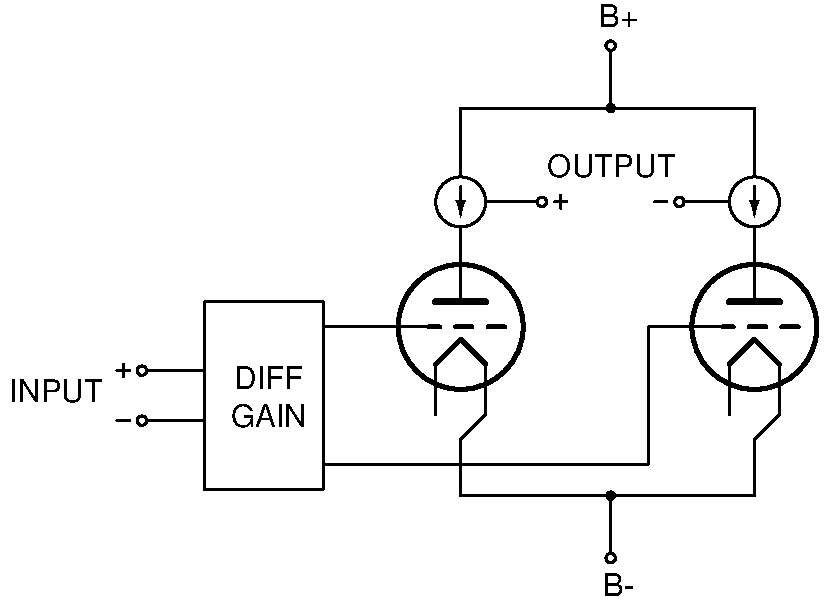
\includegraphics[width=0.7\textwidth]{OPS_concept.pdf}
\caption{Conceptual layout of the OSDEHA: differential input, gain stage stage, and push-pull DHT output stage.}
\figlabel{OPS_concept}
\end{center}
\end{figure}




%    The gyrator CCS type (as discussed by @mogliaa and others) works as a CCS in the audio/AC domain, but provides a fixed voltage at DC. This may be a useful feature to fix the DC voltages at the anodes, and hence to adjust and maintain the amplifier outputs close to 0 V.


\section{License information} \seclabel{license}
Copyright Matthias Brennwald 2024.                                                    

The OSDEHA is Open Hardware and is licensed under the CERN-OHL-S v2 or any later version.

You may redistribute and modify this source and make products using it under the terms of the CERN-OHL-S v2 (\url{https://ohwr.org/cern_ohl_s_v2.txt}).

This source is distributed WITHOUT ANY EXPRESS OR IMPLIED WARRANTY, INCLUDING OF MERCHANTABILITY, SATISFACTORY QUALITY AND FITNESS FOR A PARTICULAR PURPOSE. Please see the CERN-OHL-S v2 for applicable conditions.

Source location: \url{https://github.com/mbrennwa/OSDEHA}

As per CERN-OHL-S v2 section 4, should You produce hardware based on this source, You must where practicable maintain the Source Location visible on the external case of the OSDEHA or other products you make using this source.            

% list of references
\bibliographystyle{unsrt}
\bibliography{OSDEHA_documentation}


\end{document}
